\section{Diagrama de la Estructura General del Sistema} 
La Figura \ref{fig:Diagrama de sistemas} ilustra la arquitectura general del sistema propuesto, presentando los principales componentes que lo integran y sus interconexiones desde la perspectiva del patrón de diseño Modelo-Vista-Controlador (MVC). Este enfoque promueve la separación de responsabilidades, dividiendo la aplicación en tres partes principales:

\begin{itemize}
	\item \textbf{El Modelo (Model):} Representa la lógica de negocio, los datos de la aplicación y las reglas para manipular esos datos. Es el corazón de la aplicación, independiente de la interfaz de usuario.
	\begin{itemize}
		\item El \textbf{Servidor Java Spring-Boot} (desplegado en \textbf{Azure}) se encarga de la lógica de negocio, procesando las solicitudes, realizando validaciones, aplicando reglas de negocio y gestionando la interacción directa con la base de datos PostgreSQL mediante el protocolo SSL. Podría decirse que este servidor contiene la lógica que opera sobre el Modelo y expone los datos y funcionalidades a otros componentes (Son principalmente los Service y los Repository).
		\item El \textbf{Servidor Red Neuronal} (también en \textbf{Azure}) puede considerarse una extensión especializada del Modelo, proporcionando funcionalidades avanzadas de lógica de negocio (reconocimiento facial) que operan sobre datos y que el Controlador podría invocar para procesamientos específicos.
	\end{itemize}
	
	\item \textbf{La Vista (View):} Es la capa muestra los datos al usuario. Su responsabilidad principal es renderizar la interfaz de usuario y reflejar el estado actual del Modelo.
	\begin{itemize}
		\item El \textbf{Sistema Web (Simulación SAES y DAE)}, desplegado localmente, actúa como una Vista para los usuarios de escritorio, presentando la información y recibiendo las interacciones.
		\item La \textbf{App Móvil} representa otra Vista, diseñada específicamente para dispositivos móviles, ofreciendo una interfaz adaptada para el usuario final en un entorno portátil.
	\end{itemize}
	
	\item \textbf{El Controlador (Controller):} Actúa como un intermediario entre el Modelo y la Vista. Recibe las entradas del usuario desde la Vista, las traduce en acciones apropiadas para el Modelo, y actualiza la Vista con la respuesta del Modelo.
	\begin{itemize}
		\item En este sistema distribuido, el rol del Controlador se distribuye entre los mecanismos de comunicación de los clientes y la parte inicial de procesamiento del \textbf{Servidor Java Spring-Boot}. Cuando el Sistema Web o la App Móvil envían solicitudes a los servidores vía HTTPS, estas solicitudes actúan como ´´entradas del usuari´´.
		\item El \textbf{Servidor Java Spring-Boot} (a través de sus controladores RESTful internos) es quien recibe estas solicitudes de la Vista, invoca la lógica de negocio apropiada dentro del Modelo (o en el Servidor Red Neuronal si es necesario), y prepara los datos para ser enviados de vuelta a la Vista, completando el ciclo.
	\end{itemize}
\end{itemize}


\begin{figure}[htbp!]
	\begin{center}
		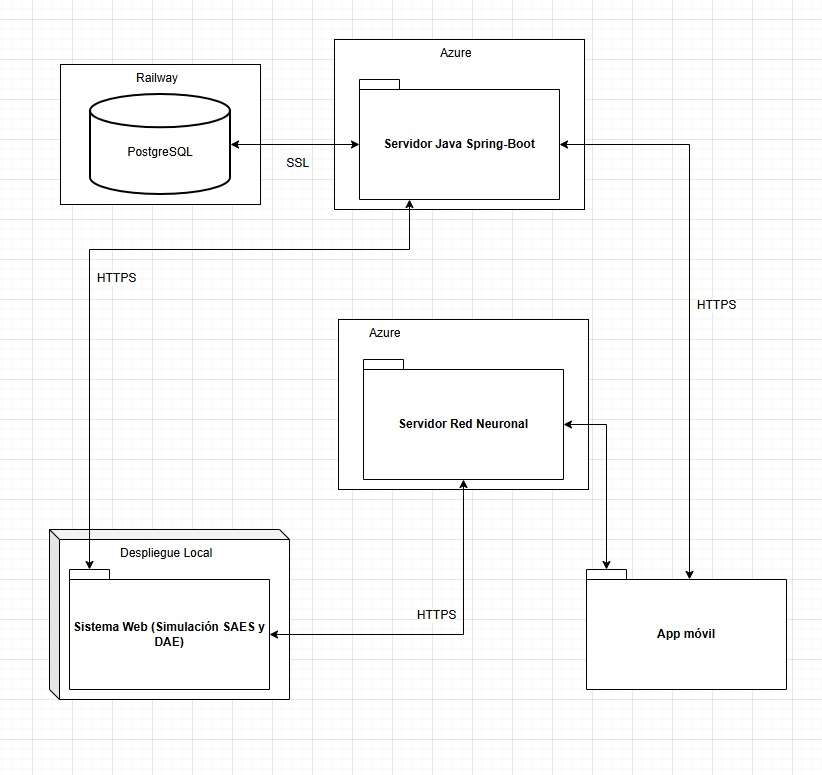
\includegraphics[width=0.8\textwidth]{images/DiagramaGeneralClases}
		\caption{Diagrama de la Estructura General del Sistema.}
		\label{fig:Diagrama de sistemas}
	\end{center}
\end{figure}

A continuación se entrara más en detalle en la estructura interna de los componentes del sistema del diagrama anterior.

\newpage